\documentclass[12pt, a4paper]{article}
\setlength{\parindent}{0pt}
\usepackage[a4paper, portrait, margin=1in]{geometry}
\usepackage{graphicx}

\graphicspath{.}

\usepackage{preamble}

\begin{document}

\textbf{Q5}

\textit{(a)}

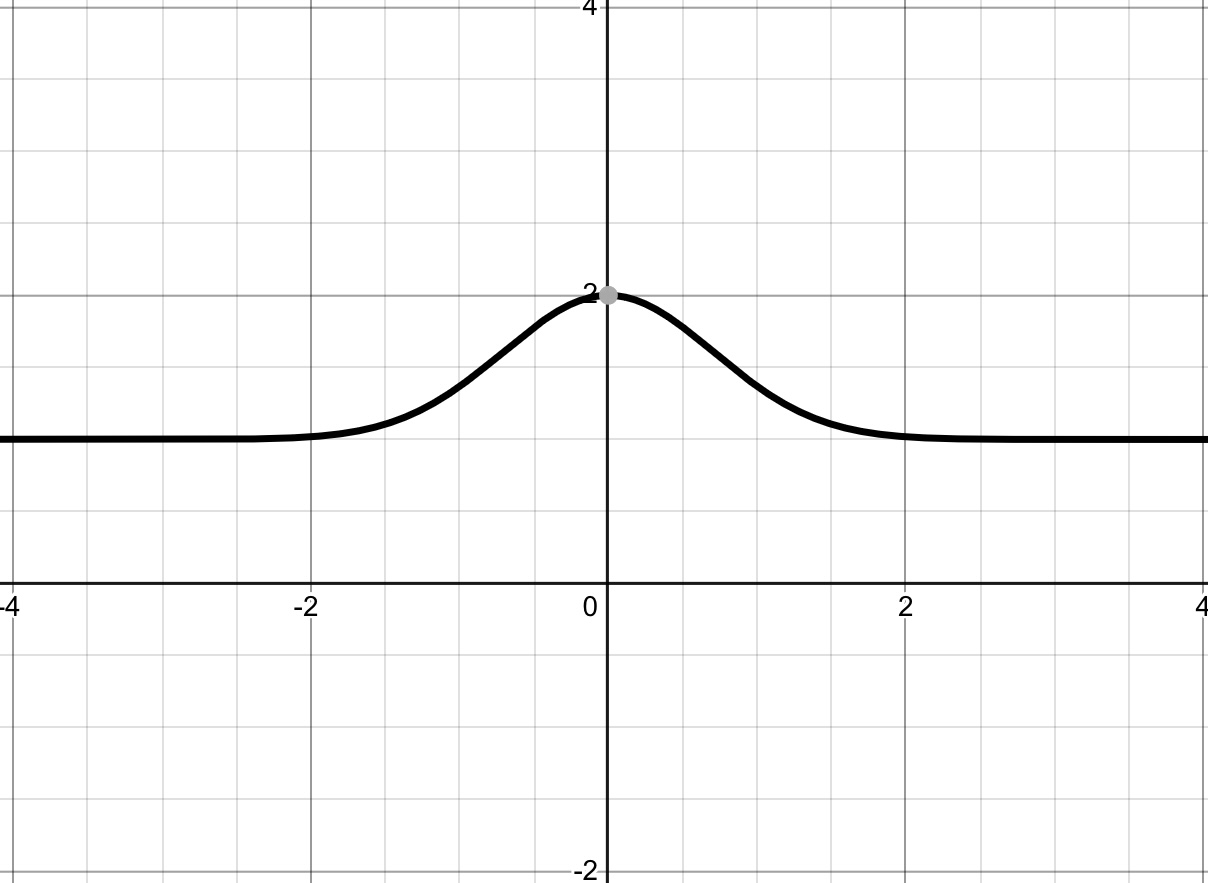
\includegraphics[height=7cm]{q5graph.jpg}

\textit{(b)}

\begin{proof}
    By properties of integrals, we observe

    \begin{align*}
        \int_0^x (e^{-t^2} + 1)\;dt & = \int_0^x (e^{-t^2}) \; dt + \int_0^x 1 \; dt\\
        & = \int_0^x (e^{-t^2} + 1) \; dt + x
    \end{align*}

    Since $e^{-t^2} > 0$ for all $t$, $\int_0^x (e^{-t^2} + 1)\;dt > x$ for $x \geq 0$.

    Then, $e^{-t^2} \leq 1 \implies e^{-t^2} + 1 \leq 2 \implies \int_0^x (e^{-t^2} + 1)\;dt \leq 2x$,
    which leaves us with

    \[
        x \leq F(x) \leq 2x
    \]
\end{proof}

\textit{(c)}

\begin{proof}
    By properties of integrals, we have

    \[
        \int_0^x (e^{-t^2} + 1)\;dt = -\int_x^0 (e^{-t^2} + 1)\;dt
    \]

    Thus for $x \leq 0$, this is simply the inverse of \textit{(b)}.
\end{proof}

\textit{(d)}

\begin{proof}
    By (b) and (c) and the Squeeze Theorem, for $x \geq 0$:

    \[
        x \leq F(x) \leq 2x \implies \inflim F(x) = \infty
    \]

    This also holds for the opposite case, $x \leq 0$.
\end{proof}

\textit{(e)} True.
\end{document}